\section{Theory}

%% Part1 - solar cells -> materials
\subsection{Solar cells}

Most solar cells made are crystalline, meaning the structure of atoms is ordered, or periodic. Generally the crystals will contain imperfections and impurities. Some solar cell materials however, is not crystalline, but are missing periodicity. These solar cells are made from amorphous materials.

\subsubsection{Bandgap}

A free electron in vacuum can posses any energy. An electron in a crystal is bound by an energy gap divided by energy positions the electrons can't possess. Every available energy state can only room two electrons according to the Pauli principle. For a crystal, the energy bands can be viewed as an overlap in between single electron energy states. This can be viewed as the crystals 'electron'-shell.

\begin{figure}[H]
 \centering
 	% Tegning
 	\begin{tikzpicture}[scale=0.5]
     	\draw[very thick,->] (1,6) -- node[below] {x}  (25,6); % X akse
    	\draw[very thick,->] (1,6) -- node[left] {\begin{sideways}Energy\end{sideways}} (1,18); % Y akse
    
    \begin{scope} % Valens og ledningsb�nd
		    \draw[thick,fill=black!10] (2,7) rectangle node {Valence band} ++(22,4);
        \draw[thick,fill=black!10] (2,13) rectangle node {Conduction band} ++(22,4);
        \draw[thick,<->] (13,13) -- node[right] {Band gap} (13,11); % Pil
    \end{scope}
    \end{tikzpicture}    \caption{Energy bands}
    \label{fig:energiband}
\end{figure}

The upper band is called conduction band, and the band right below it, is called the valence band. In between these two, are the ideally forbidden band gap. This band gap is very important in relations with solar cells, and is often given in the units of electron volts (eV).

For electrons to move out of the crystal, they have to be in the conduction band. For electrons to get to the conduction band, they need to have enough energy to move from the valence band. This can happen if the electron has enough thermal energy, or receive energy from the outside, like light. This gives the material increased conductivity. In addition to this, there will be a free state in the valence band, which results in a less probability of collisions among the remaining electron, which lead to a higher mean kinetic energy of the electrons in the valence band. This also contribute to a better conductivity for the material. 

For light to excite an electron from the valence band to the conduction band, it needs to have equal, or more energy than the band gap. Energy of light in electron volts is given by:

\begin{equation}
E=h\nu =\frac{hc}{\lambda}
\label{eq:light_energy}
\end{equation}

where $E$ is energy in electron volts, $h$ is Planks constant, $\nu$ is frequency, and $c$ is the speed of light.

Materials is often divided into three categories; Isolators, semiconductors, and conductors. Isolators have none, or few electrons in the conduction band, which gives them poor conductivity. Conductors often have filled conduction bands in room temperature, which provide good conductivity. Even at 0K, conductors have a partially filled conduction band. Semiconductors on the other hand, does not have any electrons in the conduction band at 0K. Semiconductors have lower conductivity than conductors, but better than isolators. The bandgap for semiconductors lay in between that of the conductors and isolators. At room temperature semiconductors have a partially filled conduction band.

\begin{figure}[H]
 \centering
 % Tegning
 

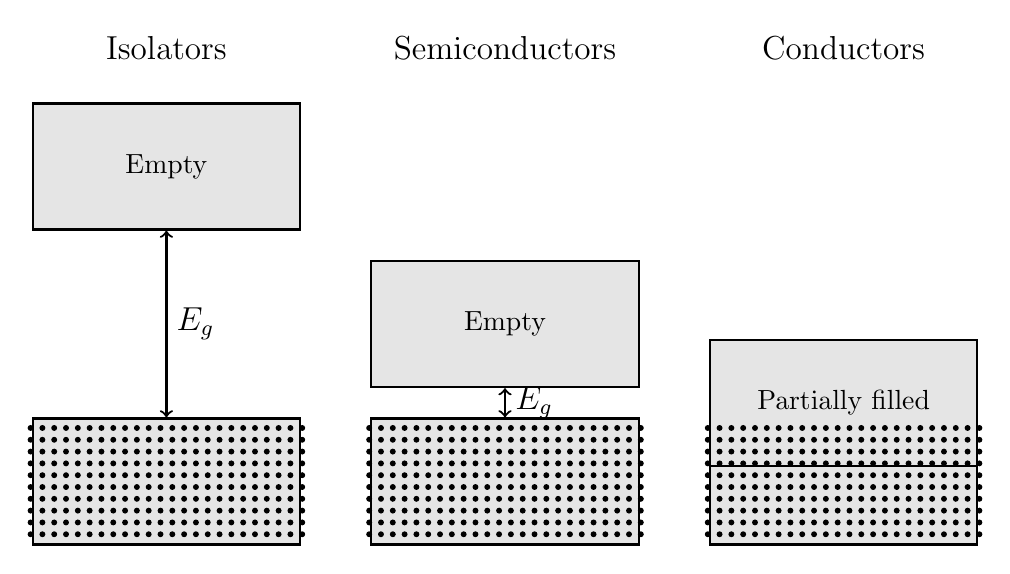
\begin{tikzpicture}
 	% Styles til elementer (kan ogs� v�re generelle utenfor tikzpicture)
	\tikzstyle{ledningsband} 	=	[rectangle, draw, thick, fill=black!10, text width=9em, text centered, minimum height=1.6cm]
	\tikzstyle{valensband}		= [rectangle, draw, thick, fill=black!10, text width=9em, text centered, minimum height=1.6cm]


	% Boksene i bunnen
	\node[valensband]	(valens_isolator)																										{};
	\node[valensband]	(valens_halvleder)	[right of=valens_isolator,  node distance=4.3cm]	{};
	\node[valensband]	(valens_metall)			[right of=valens_halvleder, node distance=4.3cm]	{};	
	
	% Boksene i toppen
	\node[ledningsband]	(lednings_isolator)		[above of=valens_isolator, 	node distance=4cm]	{Empty};
	\node[ledningsband]	(lednings_halvleder)	[above of=valens_halvleder, node distance=2cm]	{Empty};
	\node[ledningsband]	(lednings_metall)			[above of=valens_metall, 		node distance=1cm]	{Partially filled};
	
	% Piler
	\draw[thick,<->] (valens_isolator)  -- node[right] {\large $E_g$} (lednings_isolator);
	\draw[thick,<->] (valens_halvleder) -- node[right] {\large $E_g$} (lednings_halvleder);
	
	% Tekst p� toppen
	\node (isolator_tekst)  [above of=lednings_isolator,node distance=1.5cm]	{\large Isolators};
	\node (halvleder_tekst) [right of=isolator_tekst, 	node distance=4.3cm] 		{\large Semiconductors};
	\node (metaller_tekst)  [right of=halvleder_tekst, 	node distance=4.3cm] 		{\large Conductors};
	
	% Elektroner i valensb�nd
	\foreach \y in {0,0.15,...,1.4}
		\foreach \x in {0,0.15,...,3.5} {
			\draw (\x-1.725,\y-0.67) circle (0.03cm) [fill=black];	% Isolator
			\draw (\x+2.575,\y-0.67) circle (0.03cm) [fill=black];	% Halvleder
			\draw (\x+6.875,\y-0.67) circle (0.03cm) [fill=black];	% Metall
		}	
	
\end{tikzpicture}

	    \caption{Typical bandgaps at 0K} 
 \label{fig:bandgap}
\end{figure}
\vspace{10mm}

Typical bandgap for semiconductor silicon is E$_g$=1.1~eV, compared with 5~eV for diamond, which is an isolator \cite{streetman}.

Holes is a description of missing electrons in the valence band. A hole will appear when an electron is excited from the valence band into the conduction band. With a small bandgap, and high temperatures, there will be a considerably larger amount of electrons in the conduction band, compared to low temperatures, and a large bandgap. This is described by law of mass action

\begin{equation}
np=N_cN_ve^{-\frac{E_g}{kT}}
\label{eq:massevirkningsloven}
\end{equation}

where $n$ is number of electrons, $p$ is number of holes, $N_c$ and $N_v$ is constants for a given material, $E_g$ is the bandgap, $k$ is Boltzmanns constant, and $T$ is temperature in Kelvin. For an intrinsic semiconductor, meaning a semiconductor without any doping atoms, like a pure silicon crystal, the law of mass action can be written as

\begin{equation}
np=n_i^2
\label{eq:massevirkningsloven_intrinsikk}
\end{equation}

where

\begin{equation}
n_i=\sqrt{N_c N_v}e^{-\frac{E_g}{2kT}}
\label{eq:intrinsikk}
\end{equation}


\subsubsection{Doping}

By adding certain atoms of a different type than those constituting the semiconductor itself, it is possible in increase the concentration of electrons in the conduction band without a concomitant increase on the number of holes in the valence band. This is called donor-doping. An example of donor doping is added phosphorous into a silicon crystal. This will result in more electrons in the conduction band, due to phosphor having one more valence electron than silicon. The doping is usually so small that the band structure won't be affected. By adding phosphorous this way, one has increased electrons, $n$, without increasing holes, $p$. This is called donor doping. If you instead of phosphor, add boron, the material will be acceptor doped. This is due to boron having one less electron in the valence band than silicon, and would result in an extra hole in the valence band of the crystal. Usually the number of dopants in silicon are substantially larger than the intrinsic concentration, $n_i$, so that

\begin{equation}
n \approx N_d
\label{eq:donordoping}
\end{equation}

for donor doping, and

\begin{equation}
p \approx N_a
\label{eq:akseptordoping}
\end{equation}

for acceptor doping where $N_d$ is donor concentration, and $N_a$ is acceptor concentration.

A doped semiconductor is generally called extrinsic \cite{streetman}. If a semiconductor is doped with a number of donor atoms, it is called n-doped or n-type, due to there being more electrons than holes. For acceptor doping, it is called p-doped, or p-type, semiconductor. The dominating charge carrier in the semiconductor are called majority carriers. The other charge carrier, i.e. holes in the n-type semiconductor are called minority carriers.

\subsubsection{Transport and recombination processes}

There are two mechanisms that contribute to transport of electrons and holes in semiconductors: drift, and diffusion. Drift is a transport of a charge carrier due to an electric field. For transport of a hole in one dimension, the current $I_p$ is equal to the amount of holes $N_p$ times the charge $q$ crossing a cross-sectional area.

\begin{equation}
I_p = N_p q
\label{eq:drift}
\end{equation}

In vacuum, an electric field would accelerate the electrons, and the velocity would increase indefinitely. In solids, however, interactions of collisions with other species in the solid leads to a resistance towards the drift of the charged particles, and after an initial acceleration the mean velocity becomes constant in a constant electric field. This average drive velocity, denoted $v_p$ for holes, is related to the electric field $E$ through the hole mobility $�_p$

\begin{equation}
v_p = �_p E
\label{eq:electronspeed}
\end{equation}

If all the electrons is moving in the same direction, the current per area is given by

\begin{equation}
J_p = \frac{I_p}{A} = \frac{N_p q}{A} = pAv_p \frac{q}{A} = pv_p q = pq�_p E
\label{eq:hulltetthet}
\end{equation}

combined with a similar expression for electrons

\begin{equation}
J = J_p + J_n = (nq�_n + pq�_p)E = \sigma E
\label{eq:stromtetthet}
\end{equation}

where $�_n$ is the mobility for electrons,$\sigma$ is the semiconductors conductivity, and $J_n$ is the current density due to the concerted movement of electrons. It is also usual to define the resistivity of the semiconductor as the inverse of its conductivity. The current is then obtained by

\begin{equation}
I = JA = A\sigma E = \left( \frac{A\sigma}{L}\right)V = \frac{V}{R}
\label{eq:current}
\end{equation}

which is recognized as Ohm's law.


Diffusion is a transport process caused by the random motion of the diffusing particles in the medium in which they diffuse. The net transport of particles is in the opposite direction of the concentration gradient. For holes we have

\begin{equation}
N_p=-D_p\frac{dp}{dx}
\label{eq:diffusion}
\end{equation}

where the proportionality constant $D_p$ is the diffusion coefficient (m$^2$/s) for holes.

The movement of charged particles are frequently determined by the simultaneous presence of electric fields and concentration gradients. Both of the relevant transport parameters, mobilities and diffusion coefficients, will in general depend on temperature. The relation between diffusion coefficient and mobility is

\begin{equation}
\frac{D_p}{�_p}=\frac{kT}{q}
\label{eq:transport_relation}
\end{equation}

for holes, and a corresponding one exist for electrons.

\subsubsection{Excitation and recombination}

Electrons can move from one band to another directly, or indirectly. In indirect generation and recombination the electrons can employ the so-called gap-states. Such conditions will always exist in semiconductors and are related to impurities, defects in the crystal structure, boundary surfaces (grain boundaries) and surfaces. Gap-states are in between the valence band and the conduction band, which is not allowed states in a perfect crystal.


\begin{figure}[H]
\centering
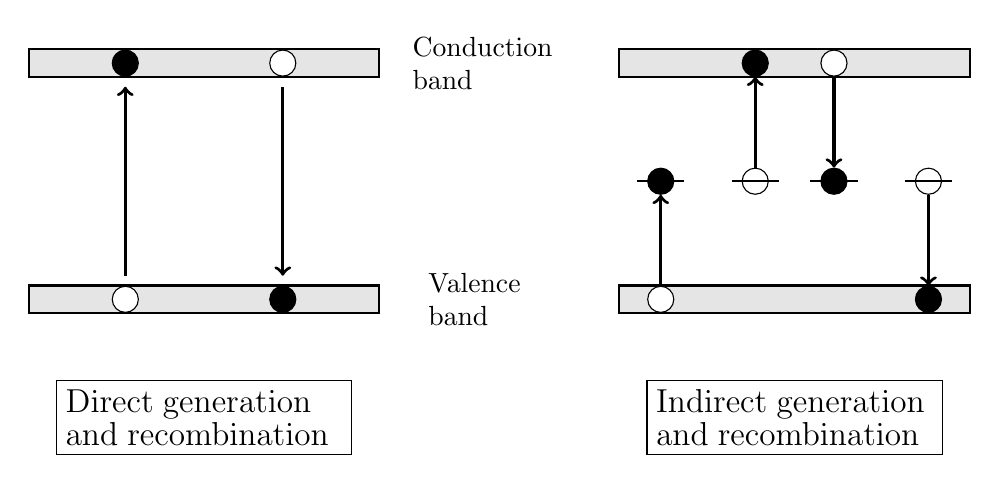
\begin{tikzpicture}

% Styles til elementer
\tikzstyle{band} 	=	[rectangle, draw, thick, text width=12em, fill=black!10, text centered, minimum height=1em]
\tikzstyle{e} 	=	[circle, draw, fill=black] % radius=0.2cm
\tikzstyle{h} 	=	[circle, draw, fill=white] % radius=0.2cm

	% Direkte
	\node[band]	(direkte_valens)																									{};
	\node[band]	(direkte_lednings)	[above of=direkte_valens, node distance=3cm]	{};
	\node[e] (elektron1) [right of=direkte_valens] {}; % Elektron
	\node[h] (hull1) [left of=direkte_valens] {}; % Hull
	\node[e] (elektron2) [left of=direkte_lednings] {}; % Elektron
	\node[h] (hull2) [right of=direkte_lednings] {}; % Hull
	\draw[very thick,->] (-1,0.3) -- (-1,2.7) {} ; % Pil opp
	\draw[very thick,<-] (1,0.3) -- (1,2.7) {} ; % Pil ned
	\node (direkte_tekst) [rectangle, draw, text width=10em, below of=direkte_valens,node distance=1.5cm]	{\large Direct generation and recombination};
	
	\node (lednings_tekst) [right of=direkte_lednings, node distance=3cm, text width=2em] {Conduction band};
	\node (valens_tekst) [right of=direkte_valens, node distance=3.2cm, text width=2em] {Valence band};
	
	% Indirekte
	\node[band]	(indirekte_valens)		[right of=direkte_valens,  node distance=7.5cm]	{};
	\node[band]	(indirekte_lednings)	[above of=indirekte_valens, node distance=3cm]	{};
	
	\node[h] (h3) [left of=indirekte_valens, node distance=1.7cm] {}; % Hull
	\node[e] (e3) [above of=h3, node distance=1.5cm] {}; % Elektron
	\draw[very thick,->] (h3) -- (e3) {}; %Pil
	\draw[thick,-] (5.5,1.5) -- (6.1,1.5) {}; % Linje gjennom
	
	\node[e] (e4) [left of=indirekte_lednings, node distance=0.5cm] {}; % Elektron
	\node[h] (h4) [below of=e4, node distance=1.5cm] {}; % Hull	
	\draw[very thick,->] (h4) -- (e4) {}; % Pil
	\draw[thick,-] (6.7,1.5) -- (7.3,1.5) {}; % Linje gjennom
	
	\node[h] (h5) [right of=indirekte_lednings, node distance=0.5cm] {}; % Hull
	\node[e] (e5) [below of=h5, node distance=1.5cm] {}; % Elektron
	\draw[very thick,->] (h5) -- (e5) {}; % Pil
	\draw[thick,-] (7.7,1.5) -- (8.3,1.5) {}; % Linje gjennom
	
	\node[e] (e6) [right of=indirekte_valens, node distance=1.7cm] {}; % Elektron
	\node[h] (h6) [above of=e6, node distance=1.5cm] {}; % Hull	
	\draw[very thick,->] (h6) -- (e6) {}; %Pil
	\draw[thick,-] (8.9,1.5) -- (9.5,1.5) {}; % Linje gjennom
	
	\node (indirekte_tekst) [rectangle, draw, text width=10em, below of=indirekte_valens,node distance=1.5cm]	{\large Indirect generation and recombination};
	
\end{tikzpicture}	

\caption{Generation and recombination}%
\label{fig:indirect}%
\end{figure}

In semiconductors with direct bandgap, like GaAs, both processes will occur. In semiconductors with with indirect bandgap, like silicon, a direct process cannot happend without contributions from lattice vibrations (phonons), something which makes the process less probable. This is one of the reasons why impurities in silicon solar cells is an important parameter. The electron in an indirect process is moving in the form of a plane wave with propagation constant $\vec{k}$, also called wave vector. 


% Indirekte b�ndbap figur
\begin{figure}[H]
\centering
\includegraphics[width=\columnwidth]{bandgap}%
\caption{Direct and indirect recombination (figure from \cite{aps})}%
\label{fig:indirect_direct}%
\end{figure}


Generation and recombination processes can be described as net flow of electrons to the conduction band, $U_n$, proportional to the deviation from equilibrium

\begin{equation}
U_n = - \frac{n-n^0}{\tau_n}
\label{eq:generation_n}
\end{equation}

where $\tau_n$ is the lifetime of electrons, which is the time that an electron of average speeds in the conduction band use before recombining with a hole. $n$ is the concentration of electrons and $n^0$ is the equilibrium concentration of electrons, $n^0=n_i^2$. Similarly, the net production of holes $U_p$

\begin{equation}
U_p = - \frac{p-p^0}{\tau_p}
\label{eq:generation_p}
\end{equation}

\subsubsection{Solar cell}

In a semiconductor with one p-doped, and one n-doped area laying next to each others is called a pn-junction. A pn-junction has rectifying properties, meaning the electrical conductance are significantly better in one direction than the other, in contrast to a resistor for which it does not matter, as the voltage drops across the resistance whether the current runs one way or another through it. This rectifying behavior defines a diode. Due to the p-side having a larger concentration of electrons in the conduction band than the n-side, there will be a net transport of conduction band electrons from the n-side, to the p-side by diffusion. The same is also happening for holes from the p-side to the n-side. This net flow of charge is called the diffusion current. In principle, the dopants of Si, B, and P can also diffuse between the two parts of the crystal. Such a transport will only be significant at the temperature range of 800 to 900$^\circ$~C, and can be neglected at  temperatures like room temperature.

% figur fra s. 14 i kompendiet

\begin{figure}[H]%
\centering
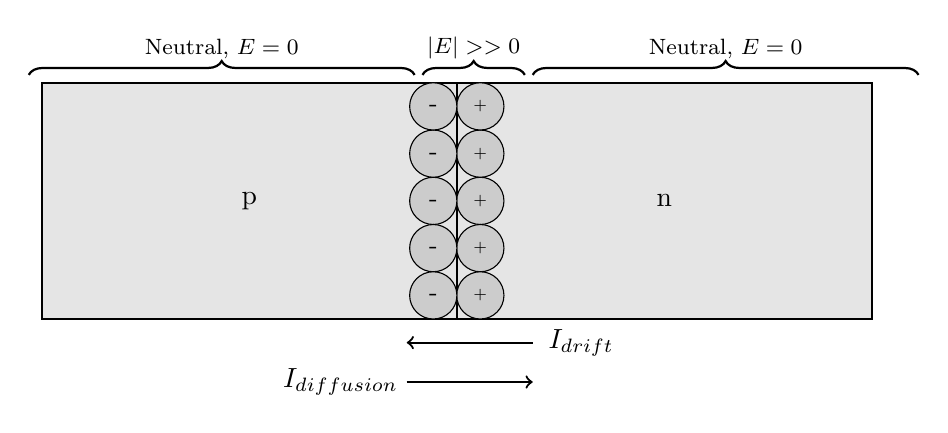
\begin{tikzpicture}

	\tikzstyle{box} 	=	[rectangle, draw, thick, fill=black!10, minimum width=15em, minimum height=3cm]
	\tikzstyle{ladning} 	=	[circle, draw, fill=black!20, minimum size=0.6cm]
	\def\edistance{0.6cm}
	
	\node[box]	(p)	{p};
	\node[box]	(n) [right of=p, node distance=15em]	{n};
	
	\node[ladning] (p3) [right of=p, node distance=8.35em] 	{\tiny{+}};
	\node[ladning] (p2) [above of=p3, node distance=\edistance] {\tiny{+}};
	\node[ladning] (p1) [above of=p2, node distance=\edistance] {\tiny{+}};
	\node[ladning] (p4) [below of=p3, node distance=\edistance] {\tiny{+}};
	\node[ladning] (p5) [below of=p4, node distance=\edistance] {\tiny{+}};
	
	\node[ladning] (n3) [left of=n, node distance=8.35em] 			{\small{-}};
	\node[ladning] (n2) [above of=n3, node distance=\edistance] {\small{-}};
	\node[ladning] (n1) [above of=n2, node distance=\edistance] {\small{-}};
	\node[ladning] (n4) [below of=n3, node distance=\edistance] {\small{-}};
	\node[ladning] (n5) [below of=n4, node distance=\edistance] {\small{-}};
	
	% Draw curly braces using path decoration
	\draw [thick,decorate,decoration={brace,amplitude=5pt}]
   (2.2,1.6) -- (3.5,1.6)
   node [black,midway,above=2pt] {\footnotesize $|E|>>0$};

	\draw [thick,decorate,decoration={brace,amplitude=5pt}]
   (-2.8,1.6) -- (2.1,1.6)
   node [black,midway,above=2pt] {\footnotesize Neutral, $E=0$};

	\draw [thick,decorate,decoration={brace,amplitude=5pt}]
   (3.6,1.6) -- (8.5,1.6)
   node [black,midway,above=2pt] {\footnotesize Neutral, $E=0$};

	% Str�mpiler
	\draw [thick,<-] (2,-1.8) -- (3.6,-1.8) node [right=2pt]	{$I_{drift}$}; 
	\draw [thick,->] (2,-2.3) -- (3.6,-2.3) node [left=45pt]	{$I_{diffusion}$}; 

\end{tikzpicture}

\caption{Depletion area}%
\label{fig:depletionarea}%
\end{figure}

Each hole that leaves the p-side will leave behind an acceptor that is no longer neutralized by a hole. Similarly, each electron in the n-side leave behind a donor that is not neutralized by an electron. A layer near the interface between the two materials with non-neutral donors on the n-side and non-neutral acceptor in the p-side will form. This layer is often called the depletion layer, since it is essentially depleted of free charge carriers. Since the n-side of the depletion layer contains non-neutral donors this side will be positively charged. The corresponding p.side will be negatively charged. These charges therefore will cause an electric field directed from n-to p-side, or a corresponding drop in electrical potential from the n-side to the p-side. This electrical potential is resulting in a drift current which is moving in the opposite direction of the diffusion current which is resulting in equilibrium, meaning zero net flow of current.

By exposing the pn-junction to light, minority carriers may be generated beyond those generated thermally. The carriers are generated by photon absorption. This generation is usually significantly greater than the drift current. A diode not exposed to light has the following current voltage characteristic:

\begin{equation}
I=|I_{drift}|e^{\frac{qV}{kT}-1}
\label{eq:diodeiv}
\end{equation}

When the diode is exposed to light, the drift current is increased, and the current voltage characteristic is changing as seen in figure \ref{fig:ivsolcelle}.

% figur fra side 22 i kompendiet
\begin{figure}[H]
\centering
\begin{tikzpicture}

	\draw [->] (-3,0) -- (3,0) node [right=5pt]	{V};  % Y-akse
	\draw [->] (0,-2) -- (0,3) node [above=5pt]	{I}; % X-akse

	% Diode
	\draw [dashed,-] (-3,-0.2) -- (-1,-0.2);
	\draw [dashed,-] (-1,-0.2) .. controls +(right:1.2cm) .. (1.5,3);
	\draw [->, >=triangle 45] (-2.5,0.5) -- node[right] {$I_{drift}$} (-2.5,0);
	\draw [->, >=triangle 45] (-2.5,-0.7) -- (-2.5,-0.2);
	
	% Solcelle
	\draw [-] (-3,-1.8) -- (-1,-1.8);
	\draw [-] (-1,-1.8) .. controls +(right:1.5cm) .. (1.5,2);
	\draw [<->, >=triangle 45] (-1.7,-1.8) -- node[right] {$I_{light}$} (-1.7,-0.2);

\end{tikzpicture}

\caption{Current-voltage characteristics for a solar cell}%
\label{fig:ivsolcelle}%
\end{figure}

For solar cells, the current going out of the cell is usually defined as positive, so that the characteristic is flipped upside-down

\begin{equation}
I=I_{light}-I_{drift}(e^{\frac{qV}{kT}-1})
\label{eq:solarcelliv}
\end{equation}

where $I_{light}$, is the current generated by the exposing light. In an open circuit the voltage is defined as 

\begin{equation}
V_{OC}=\frac{kT}{q}\ln(\frac{I_{light}}{I_{drift}}+1)
\label{eq:voc}
\end{equation}

and max power defined as

\begin{equation}
P_m=I_m V_m
\label{eq:piv}
\end{equation}

where $P_m$ is maximum power, $I_m$ is maximum current and $V_m$ is maximum voltage. Solar cell efficiency is defined as 

\begin{equation}
\eta=\frac{P_m}{P_{inn}}=FF \frac{I_{belysning} V_{OC}}{P_{inn}}
\label{eq:virkningsgrad}
\end{equation}

where FF is the fill factor is given by

\begin{equation}
FF=\frac{I_m V_m}{I_{light} V_{OC}}
\label{eq:fillfactor}
\end{equation}


% fyllfaktor figur
\begin{figure}[H]
\centering
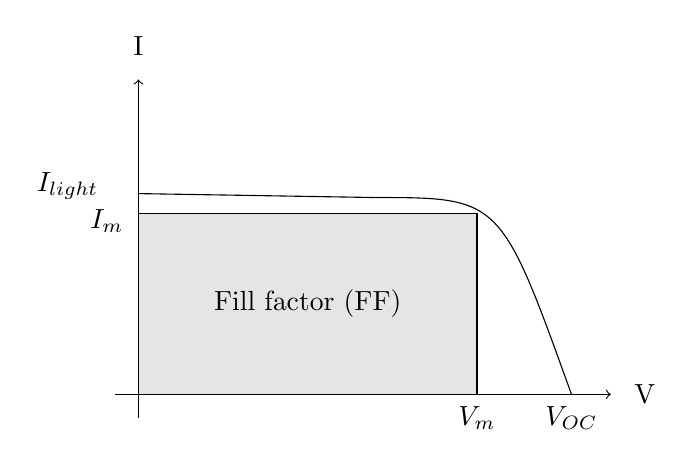
\begin{tikzpicture}

	\draw [->] (-0.3,0) -- (6,0) node [right=5pt]	{V};  % X-akse
	\draw [->] (0,-0.3) -- (0,4) node [above=5pt]	{I}; % Y-akse

	% Faktisk kurve
	\draw [-] (0,2.55) -- (3,2.5);
	\draw [-] (3,2.5) .. controls +(right:1.6cm) .. (5.5,0);
	
	% Fyllfaktor
	\node [draw, rectangle,fill=black!10,minimum height=2.3cm, minimum width=4.3cm] (FF) at (2.15,1.15) {Fill factor (FF)};
	
	% Tekst
	\node at (-0.9,2.65) {$I_{light}$};
	\node at (-0.4,2.2) {$I_m$};
	\node at (4.3,-0.3) {$V_m$};
	\node at (5.5,-0.3) {$V_{OC}$};
	
	
\end{tikzpicture}

\caption{Current-voltage characteristics with fill factor}%
\label{fig:fyllfaktor}%
\end{figure}

Solar cells with defects, have a less efficiency than clean samples

\begin{figure}[H]
\centering
\includegraphics[width=\columnwidth]{efficiency}%
\caption[I-V characteristics with defects]{A comparison of calculated I-V characteristics of three cells with 0\%, 6\%, and 15\% of area covered by defects from \cite{sopori09}.}%
\label{fig:IVwithdefects}%
\end{figure}

which makes it important to be able to characterize defects as well as impurities in order to increase solar cell efficiency.
 % Solar cells
\subsection{Material science}

A commonly used semiconductor for solar cells is silicon. The supply of silicon is practically endless. 60\% of the Earth's crust is sand, for the major part SiO$_2$. Metallurgical grade silicon (MG-Si) is produced in large amount to make special steel alloys. Its purity is only 99\% - insufficient for electronic applications \cite{solar_cells}. 

The semiconductor industry purifies this metallurgical-grade silicon until the purity is better than 99.99999\%. This corresponds to less than 0.1ppma (part per million atomic), meaning that the total number of foreign atoms must be less than 5$\cdot$10${^15}$~cm$^{-3}$, due to silicon crystalline atoms density of 5$\cdot$10$^{22}$~cm$^{-3}$ \cite{solar_cells}.

Semiconductor-grade silicon is about ten times more pure than solar-grade silicon. That means that solar-grade silicon can contain up to 1~ppma impurities and still permit reasonably efficient cells. This allows for a lower cost purification process.

\subsubsection{Czochralski method}

The most common crystallization method used for both microelectronoic and photovoltaic industries is the Czochralski (CZ) \cite{solar_cells} method shown in figure \ref{fig:czochralski_process}.

\begin{figure}[H]
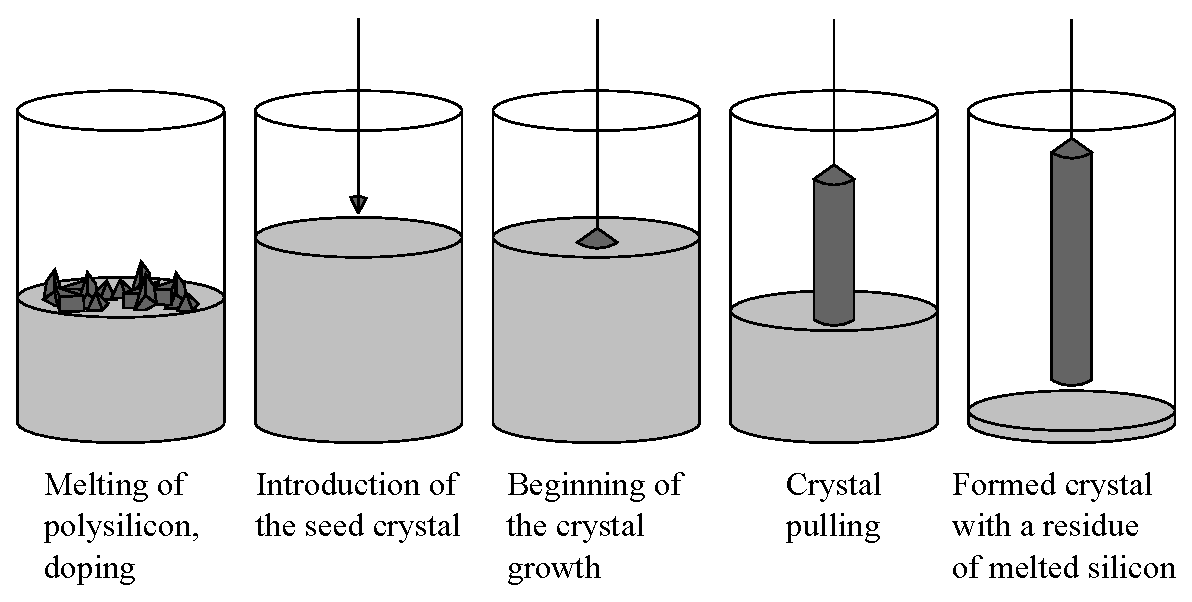
\includegraphics[width=\columnwidth]{Czochralski_Process}%
\caption{Czochralski process}%
\label{fig:czochralski_process}%
\end{figure}

In the CZ crystal growth, silicon chunks are first melted at 1414$^\circ$C in a graphite crucible lined with high purity quartz (SiO$_2$). This crucible is known as a feedstock. A small polysilicon crystal is used as a seed to start the crystallization process. The seed is carefully put in contact with the melt and then pulled out very slowly. The temperature is controlled, so that the silicon solidifies at the interface between the seed and the melt and the atoms arrange themselves according to the crystallographic structure of the seed. The crystal grows both vertically and laterally, aided by a rotation movement, yielding a cylindrical ingot of single-crystal silicon. 

The growth rate in the CZ method is about 5~cm/h and the cylindrical ingots are typically 1m long, 20~cm in diameter and 75~kg in weight \cite{solar_cells}. A disadvantage of the CZ method is that the interaction between the molten silicon and the crucible introduces some contamintants, in particular carbon and oxygen. 

\subsubsection{Float-zone process}

The highest quality silicon crystals are obtained by using the float-zone process. In this method, the starting polysilicon is first given the shape of a cylindrical bar. The bar is then locally melted by a coil using radio frequency induction. By moving the coil, and hence the molten zone, along the bar starting from the seed end, the silicon adopts the crystalline structure. The molten zone is self-supporting and is never in contact with a foreign material, thus avoiding contamination problems. The typical growth rate is 15-30~cm/h and the typical ingot is 15~cm in diameter and 1~m in length.

\subsubsection{Siemens process}

In the Siemens reactor process, trichlorosilane gas is introduced into a thermal decomposition furnace (reactor) exposing high-purity silicon rods at 1150~$^\circ$C. The trichlorosilane gas decomposes and deposits additional silicon onto the rods, enlarging them:

\begin{equation}
2 \text{HSiCl}_3 \rightarrow 2 \text{HCl} + \text{SiCl}_4
\label{eq:siemens}
\end{equation}

The silicon contained in the gas will deposit on the heated rods, which gradually grow until the desired diameter has been reached. The end product is in the form of rods or chunks of polysilicon. The technology in the Siemens reactor is widely implemented, accounting for a majority of the polysilicon production today, and produces a high purity material \cite{pv_handbook}.


\subsubsection{Multicrystalline silicon}

In order to reduce costs an increase production rates, the multicrystalline silicon (mc-Si) production method was developed. It is possible to grow silicon ingots by simply melting the starting material, typically silicon scrap, into a crucible and carefully controlling the cooling rate. Upon cooling, a directional solidification takes place and relatively large crystals grow in a columnar way. A crystalline seed is not used, and the nucleation of the silicon atoms commences in many places simultaneously, leading to a myriad of crystals (or grains) of arbitrary shape and crystallographic orientation. Each grain is several millimeters to centimeters across, an internally it has the same structure as single crystalline silicon. The boundaries between the different grains (grain boundaries), are the most obvious imperfection in the material, but they are not the only ones. Microdefect are also common and contamination from the crucible can happen as well, not to mention the possible impurities present in the starting silicon. This means that the mc-Si typically has lower electronic quality than the material produced by the CZ method. Mc-Si typically contains much less oxygen then CZ-Si. The typical crystallization rate is 3.5~kg, and the growth cycle of a complete 16~kg ingot takes 46h \cite{solar_cells}. 

\subsubsection{Wafers}

The silicon ingots have to be sliced into wafers. Before this they are shaped to meet dimensional specifications. The cylindrical CZ ingots are usually reduced to a quasi-square shape. This implies a loss of about 25\% of the material, but is necessary if a high packing factor of the cells in the module is required. The large cast silicon parallelepipeds are sawn into smaller bricks. In the case of mc-Si ingots, the shaping is also used to discard the peripheral regions that are usually heavily contaminated by the crucible, which represents approximiately 15\% of the ingot. In the photovoltaic industry the wafers are cut by a multi-wire saw machines that can cut simultaneously whole blocks, thus increasing the throughput dramatically (figure \ref{fig:wire_saw}).

\begin{figure}%
\includegraphics[width=\columnwidth]{wire_saw}%
\caption{Wafer wire saw (figure from CRS Reprocessing LLC)}%
\label{fig:wire_saw}%
\end{figure}

An abrasive slurry helps the steel wires cut through silicon, which is a very hard material. The cutting is very slow, with eight hours being typically needed to cut through a 10x10cm$^2$ block. Despite this advanced technique, slicing remains as one of the most costly steps of the whole silicon solar cell fabrication. Even if very thing wires are used approximately 30\% of the silcion is wasted as saw dust \cite{solar_cells}.


\subsubsection{Doping}

A controlled amount of boron or phosphorus is usually added to the melt (feedstock) to dope the silicon p- or n-type. Rather than the elemental boron or phosphorous, accurately measured amounts of silicon heavily doped with those elements are added to the melt. The typical boron concentration is used for solar cell applications is 1.5$\cdot$10$^{16}$~cm$^{-3}$, which results in a resistivity of 1~\ohm cm \cite{solar_cells}.


\subsubsection{Defects}

Crystals possess imperfections. They are often referred to as crystalline defects. The presence of most of these crystalline defects is undesirable in silicon wafers. Crystalline defects may be classified into four categories according to their geometry; zero-dimensional or point defects, one-dimensional or line defects, two-dimensional or area defects, and three-dimensional or volume defects

\begin{table}[H]
\begin{tabular}{|c|c|}

\hline
\textbf{Defect type} & \textbf{Examples} \\ \hline

\multirow{4}{*}{Point or zero-dimensional defects} & Vacancy defects \\
 & Interstitial defects \\
 & Frenkel defects \\
 & Extrinsic defects \\ \hline
 
\multirow{2}{*}{Line or one-dimensional defects} & Straight dislocations (edge or screw) \\
 & Dislocation loops \\ \hline
 
\multirow{3}{*}{Area or two-dimensional defects} & Stacking faults \\
 & Twins \\
 & Grain boundaries \\ \hline

\multirow{2}{*}{volume or three-dimentional defects} & Precipitates \\
 & Voids \\ \hline

\end{tabular}
\caption{Examples of crystalline defects from \cite{siliconfareast}}
\label{tab:crystalline_defects}
\end{table}

Vacancy defects are defects where a silicon atom is missing in the crystal structure. If an atom is located at a non-lattice location within the crystal, it is known as an interstitial defect. If the interstitial defect involves a silicon atom at an interstitial site within a silicon crystal, then it is referred to as a self-interstitial defect. Vacancies and self-interstitial defects are classified as intrinsic point defects \cite{siliconfareast}.
            
A Frenkel defect, is when an atom vacates its position in the crystal lattice to an interstitial position. Extrinsic point defects involve a foreign atom, and are more critical than intrinsic point defects. If this foreign atom replace a silicon atom in the lattice, it becomes a substitutional impurity. This include impurity atoms like the dopants B and P. Other common impurities are oxygen, carbon, and metals \cite{davies88}.


Dislocations, or crystal line defects consists of edge dislocations, screw dislocations or a combination of the two. Edge dislocation can be described as an extra plane of atoms squeezed into a part of the crystal lattice. The location with extra atoms would be under compressive stresses, while the part with correct number of atoms would be under tensile stresses. The line connecting all the atoms at the end of the extra plane is known as the dislocation line.

Screw dislocation is such that a step or ramp is formed by the displacement of atoms in a plane in the crystal. The dislocation line of a screw dislocation is in the axis of the screw.


\begin{figure}[H]
\centering
\subfigure[An edge dislocation]{
\includegraphics[width=.45\columnwidth]{edge_dislocation}
\label{fig:edge_dislocation}
}
\subfigure[A screw dislocation]{
\includegraphics[width=.45\columnwidth]{screw_dislocation}
\label{fig:screw_dislocation}
}
\label{fig:dislocations}
\caption{Dislocations}
\end{figure}

Dislocation loop is a closed curve consisting of an extra plane of atoms lying entirely within the crystal. The line usually form a circular shape, since this shape results in the lowest dislocation energy \cite{siliconfareast}.

Dislocations are not wanted in silicon wafers because impurities are known as recombination centers \cite{tarasov00} and serve as sinks for metallic impurities. Gettering may also occur at dislocations, which can lead to the formation of precipitates.


Stacking faults can be considered as a disturbance in the regularity of the stacking of planes in a crystal lattice. This can occur when a plane is inserted or removed from the lattice. Stacking faults can become electrically active when decorated by impurity atoms. Such stacking faults can lead to device degradation.

A twin is a mirroring of a regular lattice formed during the growth of the silicon ingot. This is usually caused by perturbation. The twin boundary is the mirror plane of the twin formation as seen in figure (\ref{fig:twin_boundary});

\begin{figure}[H]
\centering
\subfigure[Stacking faults from \cite{stacking_faults}]{
\includegraphics[width=.45\columnwidth]{stacking_fault}
\label{fig:stacking_faults}
}
\subfigure[Twin boundary]{
\includegraphics[width=.45\columnwidth]{twin_boundary}
\label{fig:twin_boundary}
}
\label{fig:dislocations_types}
\caption{Area defects}
\end{figure}

Grain boundaries are the boundary in between individual grains where crystal orientation is different from one another. This is common in mc-Si samples due to the production method.
     
Bulk or volume defects include voids and precipitates of extrinsic and intrinsic point defects. Impurities in a crystal which are introduced at a high temperature usually have a higher solubility than for lower temperatures. If the maximum concentration of an impurity allowed by its solubility at high temperature, the crystal become supersaturated with that impurity once it is cooled down. Under such supersaturated conditions, the crystal seeks and achieves equilibrium by precipitating the excess impurity atoms into another plane phase of different composition or structure. Precipitates are undesireable because they can act as sites for generation of dislocations. Precipitates can form in silicon from metallic impurities, oxygen and dopants like boron \cite{siliconfareast}.




%% Part 2 - Spectroscopy properties of Si


% band structure
% phonons
% Excitons
% EHD
% Different kinds of recombination in impurities/defects %% FIGURE (trap states, EHD, excitons etc.)
% Temperature dependance
\subsection{Spectroscopy}

When an electron hole pair is recombining, the energy is released as a photon. By measuring this photon in a photo detector it can be determined how much energy that was released during recombination. This energy tells how large the bandgap is, which in turn tells us something about the material. By shining light with high enough energy and intensity on to a sample, the light will excite electrons into all available states. When these states recombine, the emitted light can be detected by a camera as a spectra of different wavelengths. The indirect bandgap for silicon is just around 1.1~eV. This result in the energy 1.1~eV for the emitted photons. If there are impurities or defects in the silicon crystal, they can in turn emit light at different photon energies.

\begin{figure}[H]
\centering
%\includegraphics[width=10cm,bb=0 0 306 265]{luminisence.png}%
\includegraphics[width=10cm]{luminisence}%
\caption{Eksitation og recombination}%
\label{fig:luminescence}% 
\end{figure}

Figure \ref{fig:luminescence} show incoming light with high intensity in a direct bandgap material. In $a$, an electron is excited to a high energy state, which falls down to a lower energy state in $b$, after a very short time. When this electron recombines in $c$, it emits a photon with energy equal to $E_c$. Another electron is excited in $d$, which reach a so-called trap state, which can occur from impurities in the crystal, or defects. This trap state have a lower energy than the bandgap, and when this electron hole pair recombines, and lower energy is emitted. By looking at the light from such trap states, certain known spectra related to different impurities and defects can be recognized.

\subsection{Spectrometer}

In order to analyze different wavelengths, they need to be separated, and detected individually. This is done in a spectrometer. By shining light on a diffraction grating, the light is reflected at different angles by

\begin{equation}
d\sin(\theta _m)=m\lambda
\label{eq:grating_equation}
\end{equation}

where $d$ is the distance between the grating lines, $\theta _m$ is the outgoing angel of the light, $m$ is an integer denoting the diffraction order, and $\lambda$ is the wavelength. For large wavelength resolution, the angle of the reflected light will be large as well. So, in order to measure a large specter of wavelengths, several measurements with different center wavelengths is needed. This is due to physical limitations regarding the photo detector. There is a limit to how small a single pixel can be, and how long the array of pixels you can fit in the system. Each pixel translate to a separate wavelength, which measure the intensity of that wavelength only, which result in a full spectra of wavelengths and intensities. 

\subsection{Noise}

In addition to the actual photoluminescence signal, there will be noise. Noise can be from stray light in the surrounding environment hitting the camera, or it can noise from the electronics in the camera itself. Examples of noise are thermal noise, dark current, uneven amplification for different pixels in the detector, second (or more) order diffracted light from other wavelengths, background noise and different intensities for different photon energies. All measurements will be subject to noise. By having a longer integration time the signal to noise ratio is likely to increase. But a long integration time, result it a higher dark current signal. Dark current is thermally generated in the detector of the camera, and is independent of the incoming light. By cooling down the detector, the dark current noise is reduced to a minimum. This in turn makes long integration time possible, without the noise floor drowning weak signals. By blocking the signal, the dark current in addition to background noise can be measures, and then subtract this noise from the measurement containing the signal. Background noise should be fairly static, compared to dark current, and can be subtracted accurately. As for dark current, only an averaging is possible to subtract. This remaining white noise component is not possible to remove, and is clearly visible in areas without any signal. Second order diffraction can be a problem when pumping with a laser due to high intensities. Using a 532~nm laser to pump with, can result in second order diffraction at 1064~nm, which corresponds to 1.165~eV. The laser is reflected off the sample, and needs to be blocked before entering the spectrometer. However, it is possible that some light may slip through the filter, and with 532~nm pumping wavelength, the second order diffraction energy is right next to silicon bandgap which is actual signal from the photoluminescence. By using a different pumping wavelength, or having a close to perfect filter would solve this problem.

% Spectroscopy (header)
% as method
% how to cool down a sample / cryo
% What is a cryostat
% different types of cooling, He, N etc.

% Excitation of sample
% different wavelengths, give list of inntrengingsdybde for forskjellige b�lgelengder
% spot size ++

%% Part 3 - Collection of luminescence

% Optics, numerical aperture, focal plan, leses, grating/filtering, detection path components, CCD, pixel array, resolution, spatial and spectroscopy resolution (nm and ev)
\subsection{Collection of luminescence}

% Optics, numerical aperture, focal plan, leses, grating/filtering, detection path components, CCD, pixel array, resolution, spatial and spectroscopy resolution (nm and ev)

\subsubsection{Spectrometer}

In order to analyze different wavelengths, they need to be separated, and detected individually. This is done in a spectrometer. By shining light on a diffraction grating, the light is reflected at different angles by

\begin{equation}
d\sin(\theta _m)=m\lambda
\label{eq:grating_equation}
\end{equation}

where $d$ is the distance between the grating lines, $\theta _m$ is the outgoing angel of the light, $m$ is an integer denoting the diffraction order, and $\lambda$ is the wavelength. For large wavelength resolution, the angle of the reflected light will be large as well. So, in order to measure a large specter of wavelengths, several measurements with different center wavelengths is needed. This is due to physical limitations regarding the photo detector. There is a limit to how small a single pixel can be, and how long the array of pixels you can fit in the system. Each pixel translate to a separate wavelength, which measure the intensity of that wavelength only, which result in a full spectra of wavelengths and intensities. 

\subsubsection{Noise}

In addition to the actual photoluminescence signal, there will be noise. Noise can be from stray light in the surrounding environment hitting the camera, or it can noise from the electronics in the camera itself. Examples of noise are thermal noise, dark current, uneven amplification for different pixels in the detector, second (or more) order diffracted light from other wavelengths, background noise and different intensities for different photon energies. All measurements will be subject to noise. By having a longer integration time the signal to noise ratio is likely to increase. But a long integration time, result it a higher dark current signal. Dark current is thermally generated in the detector of the camera, and is independent of the incoming light. By cooling down the detector, the dark current noise is reduced to a minimum. This in turn makes long integration time possible, without the noise floor drowning weak signals. By blocking the signal, the dark current in addition to background light can be measures, and then subtract this noise from the measurement containing the signal. Background light should be consistent in regards to wavelength, compared to dark current, and can be subtracted more accurately. As for dark current, only an averaging is possible to subtract. This remaining white noise component is not possible to remove, and is clearly visible in areas without any signal. Second order diffraction can be a problem when pumping with a laser due to high intensities. Using a 532~nm laser to pump with, can result in second order diffraction at 1064~nm, which corresponds to 1.165~eV. The laser is reflected off the sample, and needs to be blocked before entering the spectrometer. However, it is possible that some light may slip through the filter, and with 532~nm pumping wavelength, the second order diffraction energy is right next to silicon bandgap which is actual signal from the photoluminescence. By using a different pumping wavelength, or having a close to perfect filter would solve this problem.


%% Part 4 - Litterature review of relevant spectra
\subsection{Literature review of relevant spectra}

\subsubsection{Dislocation photoluminescence}

Several investigations have documented that dislocations in silicon give rise to characteristic photoluminescence (PL) spectra below the band edge. First showed for low temperatures in \cite{drozdov76}, which labeled them D1 (0.812eV), D2 (0.875eV), D3 (0.934eV) and D4 (1.000eV). The samples where deformed at 850$^\circ$ C by bending, so that dislocation densities was inhomogeneous along the samples. \cite{drozdov76} states that the intensity of these lines increase closer to the dislocation-rich parts of the crystal. At the same time the intensity of the intrinsic characteristics decrease. The distance between D1-D4 (62 $\pm$ 3 meV) corresponds to the energy of the optical phonons in silicon \cite{drozdov76}. \cite{drozdov76} reports that D1 and D2 are dominant in heavily deformed Si crystals, while D3 and D4 predominate in weakly deformed Si. A similar result was also reported by recent study \cite{lee09} for small angle grain boundaries using cathodoluminescence.

It has been suggested in \cite{sauer85} that D1-D4 are due to dislocations which have been frozen in under low-shear stress. \cite{sauer85} state that photoluminescence under uniaxial stress shows that D1/D2 originate in the tetragonal defect with random orientation relative to <100> directions. \cite{sauer85} conclude that D3 and D4 are closely related, whereas the independent D1/D2 centers might be deformation-produced point defects in the strain region of dislocations. D1 and D2 is known to be closely related, as well as D3 and D4, and there have been no reports on the D-line spectrum missing only the D1 line \cite{sugimoto06}.

The origin of D1 and D2 is not clear. It has been argued that they originate in electronic transition at the geometrical kinks on dislocations \cite{suezawa83}, point defects \cite{sauer85} and impurities \cite{higgs91} and/or from the reaction products of dislocations \cite{sekiguchi95}. On the other hand, D3 and D4 lines is generally thought to be related to electronic transition within dislocation cores \cite{kveder95}. In addition, it has been suggested that the D3 line most likely is a phonon-assisted replica of D4 \cite{kveder95}.

New lines D5 and D6 emerge when high-temperature, low-stress deformation is followed by low-temperature, high-stress deformation. \cite{sauer85} propose that line D5 is due to straight dislocations and D6 is due to stacking faults. \cite{sauer85} also suggest that D3/D4 photoluminescence is much more characteristic of the dislocations themselves than the D1/D2 emission lines. \cite{weronek91} state that D5 is correlated with electron-hole recombination at localized centers on separate partial dislocations. After annealing at moderate temperatures (T > 360$^\circ$C) the new lines merge into D4 \cite{weronek91}.

Both \cite{drozdov76} and \cite{sauer85} studied plastically deformed silicon made by the Czochralski process (Cz-Si). \cite{tarasov00} studied  dislocations in multicrystalline silicon (mc-Si) and found similar lines with the entire set of D-lines shifted with around 10meV, presumably due to a strain field. Using a laser annealing technique \cite{staiger94}, introducing dislocations on a Cz-Si wafer, confirm the band location of D1-D4 from \cite{sauer85} in \cite{tarasov00}. A principal difference between dislocation D'-lines in mc-Si versus D-lines in Cz-Si is a substantial broadening in regards to energy (60-70meV at 77K) of the D1'/D2' lines observed in mc-Si \cite{tarasov00}.

\begin{table}[H]
\centering
\begin{tabular}{|c|c|c|c|c|}
\hline
Cz-Si \cite{drozdov76} & D1 & D2 & D3 & D4 \\
	& 0.812eV & 0.875eV & 0.934eV & 1.000eV \\
\hline
mc-Si \cite{tarasov00} & D1' & D2' & D3' & D4' \\
		& 0.80eV & 0.89eV & 0.95eV & 1.00eV \\
\hline
\end{tabular}
\caption{Energy positions of dislocation D-lines in Cz-Si and D' bands in mc-Si}
\label{tarasovlines}
\end{table}

Photoluminescence mapping in \cite{tarasov00} of the 0.78eV (0.8eV) band intensity reveal a linkage to areas of a high dislocation density. This band should also be visible in room temperature \cite{tarasov00}. \cite{tarasov00} also reveal a linear dependence of the band-to-band photoluminescence intensity and minority carrier lifetime across entire multicrystalline-Si wafers.

Dislocation related lines (D-lines) has been observed in low temperature photoluminescence spectra from the regions which included the intragrain defects. \cite{sugimoto06} concluded that grain boundaries are not active recombination centers. \cite{sugimoto06} also show a TO-phonon replica of the boron bound exiton at 1.093eV. Intensity of boron bound exciton from the long lifetime regions was higher than that from the short lifetime regions. D-lines reported by \cite{sauer85} are in a short lifetime region. For a long lifetime region, \cite{sugimoto06} observe a peak at 1.00eV which is not the D4 line, but the zone center optical phonon sideband of the two-hole transition in the boron bound exciton \cite{dean67}. \cite{kitler02} conclude that a relatively low contamination level of dislocations in the order of 10 impurity atoms/mm of the dislocation length produces D1 defect luminescence at room temperature and also degrades both the band-to-band luminescence and minority-carrier diffusion length.

It is believed that the intra-grain defects observed in the photoluminescence mapping are dislocations decorated with the heavy metals \cite{sugimoto06}. \cite{tarasov01} found that if the contamination level is too low, or too high (dislocation decorated by metal silicate precipitates) the defect photoluminescence band vanished in room temperature. However, a relatively low contamination level of dislocations, in the order of 10 impurity atoms per micron of the dislocation length produces distinguishable defect band luminescence \cite{tarasov01,kitler02}. 

\cite{sugimoto07} conclude that defects are metal contaminated dislocation clusters which originated from small angle grain boundaries. \cite{sugimoto07} study origins of the defects by low temperature photoluminescence spectroscopy, electron backscatter diffraction pattern measurement and the etch-pit observation. \cite{arguirov07} demonstrate three areas of a sample with only D3 and D4 present, and conclude that this is due low concentration of metallic impurities.

\subsection{Impurities}

Diffusion of transition metals into silicon crystals result in a variety of different electrically active levels in the forbidden bandgap. Impurities is also known to create precipitates inside a silicon crystal, which change the photoluminescence spectra compared to interstitial impurities.

There are several units of impurities in silicon that's commonly used. Examples are: ppbw (Parts Per Billion by Weight), ppba (Parts per Billion Atomic ) and atoms/$cm^3$. To convert from ppbw to atoms/$cm^3$, the following equation can be used:

\begin{equation}
atoms/cm^{-3} = 10^{-9} [ppbw] \cdot N_A \cdot [density(Si)] / [atomic mass of element]
\label{eq:ppbw}
\end{equation}

where N$_A$ is Avogradro's number, density(Si) is in g/cm$^3$, and atomic mass is in g/mol. To convert from ppba to ppbw:

\begin{equation}
ppbw = [atomic mass of element] / [atomic mass of Si]
\label{eq:ppba}
\end{equation}

% 'pure' impurities
\subsubsection{Atom impurities}

Early work done by \cite{dean67} compare intrinsic silicon from the Czochralski process with doped silicon. \cite{dean67} do extensive photoluminescence study with doping atoms As, P, Sb, Bi, B, Ga, In and Al. The high intensity transverse optical lines occur at 1.0907eV, 1.0916eV, 1.0921eV, 1.0888eV, 1.0924eV, 1.0914eV, 1.0835eV and ~1.092eV respectively with the different doping atoms present. Impurities like carbon complexes with many impurities in silicon, resulting in a large variety of photoluminescence centers. Detected complexes are another C atom, one oxygen atom, one N atom, one Ga atom, the four-lithium atom complex, beryllium and numerous radiation damage centres, especially involving oxygen \cite{davies88}. See appendix \ref{energy_bands} for energies.

Doping atoms give rise to different characteristics in the photoluminescence spectra aswell. Boron doping exhibits a line right below the silicon bandgap. That particular peak is hard to detect due to a strong luminescence from the silicon itself, but its phonon replicas can be identified (figure \ref{fig:boronSiPL}). Phosphorous doping give rise to a line just below the boron line (figure \ref{fig:PSiPL}). 

Some impurities does not result in any specific photoluminescence spectra, like interstitial chromium \cite{conzelmann82}. Atleast not for wavelengths up to 1800nm. However, chromium bound with a boron atom can be identified as a peak around 0.85eV where the intensity increase linearly with laser power \cite{conzelmann82,conzelmann83}. Photoluminescence from another impurity, titanium, has been observed around 2.85eV in 4H silicon carbide by \cite{patrick74}, and in 6H by \cite{kemenade74} at 2.79eV, 2.82eV and 2.86eV named ABC lines (figure \ref{fig:Ti4HSiC}). These energies are far beyond that of the silicon bandgap, and can in cases described above, be uniquely identified.

Many of the other identified impurities are located just below the silicon bandgap in the photoluminescence spectra. Spectra for a silicon sample with a low amount of impurities can be seen in figure \ref{fig:SiPL}. Copper doping of silicon crystals results in an intense emission at 1.014eV \cite{weber82}. \cite{weronek91} study Cu doped Si and also observe a shoulder on the D1 line which presumably arises from Cu precipitates at the dislocation.

Another important impurity is iron. \cite{calao88} observe a spectrum of 0.735eV, which relate to a complex defect containing iron. Here the sample was introduced with Fe atoms into a float-zone silicon crystal (PL at figure \ref{fig:FeSiPL}). An earlier study \cite{mohring83}, observe a luminescence spectra around 1.07eV in boron-doped, iron-diffused crystalline silicon and suggest the source is Fe-B pairs. Interstitial iron Fe, is about 10 times more effective as a recombination center than Fe-B pairs by low-level lifetime measurements and therefore reduces the minority carrier diffusion length more strongly (PL at figure \ref{fig:FeBSiPL}) \cite{zoth90}.

Recent work in \cite{gundel09} show that micro-photoluminescence is an excellent tool for identifying metal precipitates in silicon as seen in figure \ref{fig:gundel_iron_precipitates}. Iron images in \cite{macdonald08} reveal internal gettering of iron to grain boundaries and dislocated regions during ingot growth. The minimum size for detection is 1$�$m, or even smaller, since the photoluminescence signal might be broadened. Precipitates from Fe and Cu are detected due to reduced band to band recombination intensity. Iron in silicon also affect the defect photoluminescence \cite{gundel09}.




% interaction with dislocations
\subsubsection{Interaction with dislocations}

Investigation in \cite{higgs92} show that transition-metal contamination plays an important role in the production of D-band luminescence from silicon samples containing either epitaxial stacking faults or oxidation-induced stacking faults. \cite{staiger94} found that Cu doping resulted in reduced intensity of D1 and D2, and the intensity of D3 and D4 become very small. \cite{weronek91} demonstrate that a complete passivation of the D-band luminescence is achieved at higher Cu and Fe concentration when deliberately contaminating high purity silicon samples which contain dislocations. However impurities like Ni, lead to no detectable changes in the spectrum \cite{weronek91}. D-band recombination in Si is found to be independent of impurities trapped at dislocations \cite{weronek91}, and \cite{sekiguchi95} concluded that metallic impurities don't seem to be related to D1 and D2 luminescence. Even so, it is still generally accepted that metal impurity influence it. Metal precipitation at crystal defects during the crystal growth can clean grains from impurities, and thus improve the performance as suggested for iron in \cite{bailey93}. A recent example of interaction with defects is iron precipitates in \cite{gundel09}, showing an enhanced defect photoluminescence at 1.3$�$m (0.95eV). The same study show that copper contamination almost completely suppress the defect photoluminescence. This is in agreement with \cite{staiger94}. Supression of defect photoluminescence by high copper concentrations was also reported in \cite{lightowlers93}. Cu precipitates can be located by  reduced intensity of the band to band photoluminescence peak, both in areas with dislocations, and without \cite{gundel09}. 

\begin{figure}%
\centering
\includegraphics[width=8cm]{gundel_iron_precipitates}%
\caption[Iron precipitates]{Bottom: Scheme of the sample preparation with the polished angle. Top: A Intensity of the BB PL peak at room temperature (a), and of the iron X-ray K$\alpha$ fluorecence (b) from \cite{gundel09}. The dislocation network intersects the surface to the right of the dashed blue line. The white circles show recombination active precipitates.}
\label{fig:gundel_iron_precipitates}%
\end{figure}

Electron hole droplets (EHD), free excitons (FE) and bound excitons (BE) localized on phosphorus atoms has been steadily observed in \cite{drozdov03} with photoluminescence on samples with low-dislocated regions. When increasing dislocation density the FE, BE and EHD bands decrease sharply. This may be due exciton capture by dislocation lines D1,D2 and non-radiative recombination \cite{drozdov03}. EHD photoluminescence intensity is highly dependent on the pumping power \cite{satoshi04}. There is a linear dependence, and pumping with 3mW or less makes it hardly visible in \cite{satoshi04}.

D1 line is shifted towards higher energies under uniaxial elastic deformation of samples with introduced dislocations or after their annealing in oxygen at 750�C \cite{drozdov81}. Room temperature mapping of the 0.77eV band is attributed to oxygen precipitates in in thermally treated silicon made by the Czochralski process (Cz-Si) \cite{tajima95}. The increase of this band on the dislocation lines is due to the preferential precipitation of oxygen \cite{tajima95}. Later, \cite{inoue07} state that the deep-level emission from multicrystalline silicon with an intensity maximum at 0.78eV at room temperature is different from that of the D1 line at low temperature. Furthermore, \cite{inoue07} suggest that the 0.78eV emission is associated with oxygen precipitation, and that the intra-grain defects are dislocation clusters decorated with oxygen impurities in addition to heavy-metal impurities. \cite{gundel08} state that the origin of trap densities in multicrystalline silicon could be structural crystal defects, which are highly decorated with oxygen precipitates.



%\subsection{Material science}

A commonly used semiconductor for solar cells is silicon. The supply of silicon is practically endless. 60\% of the Earth's crust is sand, for the major part SiO$_2$. Metallurgical grade silicon (MG-Si) is produced in large amount to make special steel alloys. Its purity is only 99\% - insufficient for electronic applications \cite{solar_cells}. 

The semiconductor industry purifies this metallurgical-grade silicon until the purity is better than 99.99999\%. This corresponds to less than 0.1ppma (part per million atomic), meaning that the total number of foreign atoms must be less than 5$\cdot$10${^15}$~cm$^{-3}$, due to silicon crystalline atoms density of 5$\cdot$10$^{22}$~cm$^{-3}$ \cite{solar_cells}.

Semiconductor-grade silicon is about ten times more pure than solar-grade silicon. That means that solar-grade silicon can contain up to 1~ppma impurities and still permit reasonably efficient cells. This allows for a lower cost purification process.

\subsubsection{Czochralski method}

The most common crystallization method used for both microelectronoic and photovoltaic industries is the Czochralski (CZ) \cite{solar_cells} method shown in figure \ref{fig:czochralski_process}.

\begin{figure}[H]
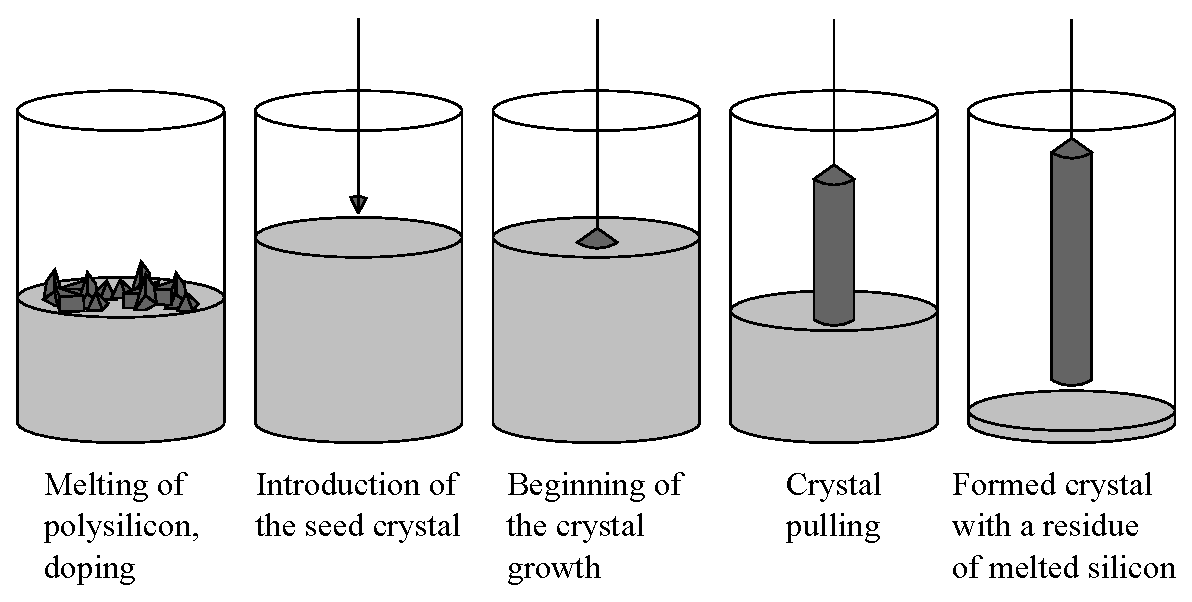
\includegraphics[width=\columnwidth]{Czochralski_Process}%
\caption{Czochralski process}%
\label{fig:czochralski_process}%
\end{figure}

In the CZ crystal growth, silicon chunks are first melted at 1414$^\circ$C in a graphite crucible lined with high purity quartz (SiO$_2$). This crucible is known as a feedstock. A small polysilicon crystal is used as a seed to start the crystallization process. The seed is carefully put in contact with the melt and then pulled out very slowly. The temperature is controlled, so that the silicon solidifies at the interface between the seed and the melt and the atoms arrange themselves according to the crystallographic structure of the seed. The crystal grows both vertically and laterally, aided by a rotation movement, yielding a cylindrical ingot of single-crystal silicon. 

The growth rate in the CZ method is about 5~cm/h and the cylindrical ingots are typically 1m long, 20~cm in diameter and 75~kg in weight \cite{solar_cells}. A disadvantage of the CZ method is that the interaction between the molten silicon and the crucible introduces some contamintants, in particular carbon and oxygen. 

\subsubsection{Float-zone process}

The highest quality silicon crystals are obtained by using the float-zone process. In this method, the starting polysilicon is first given the shape of a cylindrical bar. The bar is then locally melted by a coil using radio frequency induction. By moving the coil, and hence the molten zone, along the bar starting from the seed end, the silicon adopts the crystalline structure. The molten zone is self-supporting and is never in contact with a foreign material, thus avoiding contamination problems. The typical growth rate is 15-30~cm/h and the typical ingot is 15~cm in diameter and 1~m in length.

\subsubsection{Siemens process}

In the Siemens reactor process, trichlorosilane gas is introduced into a thermal decomposition furnace (reactor) exposing high-purity silicon rods at 1150~$^\circ$C. The trichlorosilane gas decomposes and deposits additional silicon onto the rods, enlarging them:

\begin{equation}
2 \text{HSiCl}_3 \rightarrow 2 \text{HCl} + \text{SiCl}_4
\label{eq:siemens}
\end{equation}

The silicon contained in the gas will deposit on the heated rods, which gradually grow until the desired diameter has been reached. The end product is in the form of rods or chunks of polysilicon. The technology in the Siemens reactor is widely implemented, accounting for a majority of the polysilicon production today, and produces a high purity material \cite{pv_handbook}.


\subsubsection{Multicrystalline silicon}

In order to reduce costs an increase production rates, the multicrystalline silicon (mc-Si) production method was developed. It is possible to grow silicon ingots by simply melting the starting material, typically silicon scrap, into a crucible and carefully controlling the cooling rate. Upon cooling, a directional solidification takes place and relatively large crystals grow in a columnar way. A crystalline seed is not used, and the nucleation of the silicon atoms commences in many places simultaneously, leading to a myriad of crystals (or grains) of arbitrary shape and crystallographic orientation. Each grain is several millimeters to centimeters across, an internally it has the same structure as single crystalline silicon. The boundaries between the different grains (grain boundaries), are the most obvious imperfection in the material, but they are not the only ones. Microdefect are also common and contamination from the crucible can happen as well, not to mention the possible impurities present in the starting silicon. This means that the mc-Si typically has lower electronic quality than the material produced by the CZ method. Mc-Si typically contains much less oxygen then CZ-Si. The typical crystallization rate is 3.5~kg, and the growth cycle of a complete 16~kg ingot takes 46h \cite{solar_cells}. 

\subsubsection{Wafers}

The silicon ingots have to be sliced into wafers. Before this they are shaped to meet dimensional specifications. The cylindrical CZ ingots are usually reduced to a quasi-square shape. This implies a loss of about 25\% of the material, but is necessary if a high packing factor of the cells in the module is required. The large cast silicon parallelepipeds are sawn into smaller bricks. In the case of mc-Si ingots, the shaping is also used to discard the peripheral regions that are usually heavily contaminated by the crucible, which represents approximiately 15\% of the ingot. In the photovoltaic industry the wafers are cut by a multi-wire saw machines that can cut simultaneously whole blocks, thus increasing the throughput dramatically (figure \ref{fig:wire_saw}).

\begin{figure}%
\includegraphics[width=\columnwidth]{wire_saw}%
\caption{Wafer wire saw (figure from CRS Reprocessing LLC)}%
\label{fig:wire_saw}%
\end{figure}

An abrasive slurry helps the steel wires cut through silicon, which is a very hard material. The cutting is very slow, with eight hours being typically needed to cut through a 10x10cm$^2$ block. Despite this advanced technique, slicing remains as one of the most costly steps of the whole silicon solar cell fabrication. Even if very thing wires are used approximately 30\% of the silcion is wasted as saw dust \cite{solar_cells}.


\subsubsection{Doping}

A controlled amount of boron or phosphorus is usually added to the melt (feedstock) to dope the silicon p- or n-type. Rather than the elemental boron or phosphorous, accurately measured amounts of silicon heavily doped with those elements are added to the melt. The typical boron concentration is used for solar cell applications is 1.5$\cdot$10$^{16}$~cm$^{-3}$, which results in a resistivity of 1~\ohm cm \cite{solar_cells}.


\subsubsection{Defects}

Crystals possess imperfections. They are often referred to as crystalline defects. The presence of most of these crystalline defects is undesirable in silicon wafers. Crystalline defects may be classified into four categories according to their geometry; zero-dimensional or point defects, one-dimensional or line defects, two-dimensional or area defects, and three-dimensional or volume defects

\begin{table}[H]
\begin{tabular}{|c|c|}

\hline
\textbf{Defect type} & \textbf{Examples} \\ \hline

\multirow{4}{*}{Point or zero-dimensional defects} & Vacancy defects \\
 & Interstitial defects \\
 & Frenkel defects \\
 & Extrinsic defects \\ \hline
 
\multirow{2}{*}{Line or one-dimensional defects} & Straight dislocations (edge or screw) \\
 & Dislocation loops \\ \hline
 
\multirow{3}{*}{Area or two-dimensional defects} & Stacking faults \\
 & Twins \\
 & Grain boundaries \\ \hline

\multirow{2}{*}{volume or three-dimentional defects} & Precipitates \\
 & Voids \\ \hline

\end{tabular}
\caption{Examples of crystalline defects from \cite{siliconfareast}}
\label{tab:crystalline_defects}
\end{table}

Vacancy defects are defects where a silicon atom is missing in the crystal structure. If an atom is located at a non-lattice location within the crystal, it is known as an interstitial defect. If the interstitial defect involves a silicon atom at an interstitial site within a silicon crystal, then it is referred to as a self-interstitial defect. Vacancies and self-interstitial defects are classified as intrinsic point defects \cite{siliconfareast}.
            
A Frenkel defect, is when an atom vacates its position in the crystal lattice to an interstitial position. Extrinsic point defects involve a foreign atom, and are more critical than intrinsic point defects. If this foreign atom replace a silicon atom in the lattice, it becomes a substitutional impurity. This include impurity atoms like the dopants B and P. Other common impurities are oxygen, carbon, and metals \cite{davies88}.


Dislocations, or crystal line defects consists of edge dislocations, screw dislocations or a combination of the two. Edge dislocation can be described as an extra plane of atoms squeezed into a part of the crystal lattice. The location with extra atoms would be under compressive stresses, while the part with correct number of atoms would be under tensile stresses. The line connecting all the atoms at the end of the extra plane is known as the dislocation line.

Screw dislocation is such that a step or ramp is formed by the displacement of atoms in a plane in the crystal. The dislocation line of a screw dislocation is in the axis of the screw.


\begin{figure}[H]
\centering
\subfigure[An edge dislocation]{
\includegraphics[width=.45\columnwidth]{edge_dislocation}
\label{fig:edge_dislocation}
}
\subfigure[A screw dislocation]{
\includegraphics[width=.45\columnwidth]{screw_dislocation}
\label{fig:screw_dislocation}
}
\label{fig:dislocations}
\caption{Dislocations}
\end{figure}

Dislocation loop is a closed curve consisting of an extra plane of atoms lying entirely within the crystal. The line usually form a circular shape, since this shape results in the lowest dislocation energy \cite{siliconfareast}.

Dislocations are not wanted in silicon wafers because impurities are known as recombination centers \cite{tarasov00} and serve as sinks for metallic impurities. Gettering may also occur at dislocations, which can lead to the formation of precipitates.


Stacking faults can be considered as a disturbance in the regularity of the stacking of planes in a crystal lattice. This can occur when a plane is inserted or removed from the lattice. Stacking faults can become electrically active when decorated by impurity atoms. Such stacking faults can lead to device degradation.

A twin is a mirroring of a regular lattice formed during the growth of the silicon ingot. This is usually caused by perturbation. The twin boundary is the mirror plane of the twin formation as seen in figure (\ref{fig:twin_boundary});

\begin{figure}[H]
\centering
\subfigure[Stacking faults from \cite{stacking_faults}]{
\includegraphics[width=.45\columnwidth]{stacking_fault}
\label{fig:stacking_faults}
}
\subfigure[Twin boundary]{
\includegraphics[width=.45\columnwidth]{twin_boundary}
\label{fig:twin_boundary}
}
\label{fig:dislocations_types}
\caption{Area defects}
\end{figure}

Grain boundaries are the boundary in between individual grains where crystal orientation is different from one another. This is common in mc-Si samples due to the production method.
     
Bulk or volume defects include voids and precipitates of extrinsic and intrinsic point defects. Impurities in a crystal which are introduced at a high temperature usually have a higher solubility than for lower temperatures. If the maximum concentration of an impurity allowed by its solubility at high temperature, the crystal become supersaturated with that impurity once it is cooled down. Under such supersaturated conditions, the crystal seeks and achieves equilibrium by precipitating the excess impurity atoms into another plane phase of different composition or structure. Precipitates are undesireable because they can act as sites for generation of dislocations. Precipitates can form in silicon from metallic impurities, oxygen and dopants like boron \cite{siliconfareast}.


